\documentclass[10pt,portrait, twocolumn]{article}
\usepackage{multicol}
\usepackage{calc}
\usepackage[portrait]{geometry}
\usepackage{amsmath,amsthm,amsfonts,amssymb}
\usepackage{times}
\usepackage{color,graphicx,overpic}
\graphicspath{ {images/} }
\usepackage{hyperref}
\usepackage{pgfplots}
\usepackage{esint}
\usepackage{bm}
\usepackage{tikz}
\usepackage{relsize}
\usepackage{datetime}
\usepackage{circuitikz}
\usepackage[utf8] {inputenc}
\usepackage[spanish, activeacute] {babel}
\usepackage{IEEEtrantools}
\usetikzlibrary{arrows}

\usepackage{framed}

\usepackage{pdflscape}

%Evita errores con el paquete de español y escribir flechas entre tikz nodos
\tikzset{
every picture/.append style={
  execute at begin picture={\deactivatequoting},
  execute at end picture={\activatequoting}
  }
}

\usepackage{draftwatermark}
\SetWatermarkText{Javier de Martín}
\SetWatermarkScale{0.8}

% This sets page margins to .5 inch if using letter paper, and to 1cm
% if using A4 paper. (This probably isn't strictly necessary.)
% If using another size paper, use default 1cm margins.
\geometry{top=.5cm,left=.5cm,right=.5cm,bottom=.5cm}
    
\pgfplotsset{
    dirac/.style={
        mark=triangle*,
        mark options={scale=2},
        ycomb,
        scatter,
        visualization depends on={y/abs(y)-1 \as \sign},
        scatter/@pre marker code/.code={\scope[rotate=90*\sign,yshift=-2pt]}
    }
}

% Turn off header and footer
\pagestyle{empty}

% Redefine section commands to use less space
\makeatletter
\renewcommand{\section}{\@startsection{section}{1}{0mm}%
                                {-1ex plus -.5ex minus -.2ex}%
                                {0.5ex plus .2ex}%x
                                {\normalfont\large\bfseries}}
\renewcommand{\subsection}{\@startsection{subsection}{2}{0mm}%
                                {-1explus -.5ex minus -.2ex}%
                                {0.5ex plus .2ex}%
                                {\normalfont\normalsize\bfseries}}
\renewcommand{\subsubsection}{\@startsection{subsubsection}{3}{0mm}%
                                {-1ex plus -.5ex minus -.2ex}%
                                {1ex plus .2ex}%
                                {\normalfont\small\bfseries}}
\makeatother

\newcommand{\Lagr}{\mathcal{L}}

% Define BibTeX command
\def\BibTeX{{\rm B\kern-.05em{\sc i\kern-.025em b}\kern-.08em
    T\kern-.1667em\lower.7ex\hbox{E}\kern-.125emX}}

% Don't print section numbers
\setcounter{secnumdepth}{0}


\setlength{\parindent}{0pt}
\setlength{\parskip}{0pt plus 0.5ex}

%My Environments
\newtheorem{example}[section]{Example}
% ---------------------------------------------------------------

\begin{document}


\begin{framed}
	\begin{center}
    	\Large{\underline{Sistemas de Radiocomunicación}} \\
	\large{Primera Parte} \\
    	\scriptsize{3º Ingeniería de Telecomunicaciones | UPV/EHU}\\
     	%Actualizado por última vez el \today \\
     	"\textsl{Under-promise and over-deliver}." \\
     	%\hspace{5 pt} \\
     	\small{\textbf{Javier de Martín -- 2016}}
	\end{center}
\end{framed}

%%%%%%%%%%%%%%%%%%%%%%%%%%%%%%%%%%%%%%%%%%%%%%%%%%%%%%%%%%%%%%%%%
% Tema 4

\section{\underline{1. Ingeniería del Espectro Radioeléctrico}}

\textbf{Radiocomunicación}: Telecomunicación basada en ondas de radio.\\
\textbf{Telecomunicación}: Cualquier transmisión o recepción de información por aire, radio, cable o cualquier otro sistema de electromagnetismo.\\
\textbf{Radio}: Término general aplicado al uso de ondas de radio.\\
\textbf{Ondas de Radio}: Ondas EM con frecuencias arbitrariamente menores a 3000 GHz (excepto la luz), que se propaga en el espacio sin necesidad de guías artificiales.

El espectro de radio varía desde los 3kHz hasta los 300GHz

Bandas de frecuencia según EBU (European Broadcasting Union)

	\begin{center}
\begin{tabular}{|l|l|}
\hline
Banda I   & 41-68MHz    \\ \hline
Banda II  & 87,5-108MHz \\ \hline
Banda III & 162-230MHz  \\ \hline
Banda IV  & 470-582MHz  \\ \hline
Banda V   & 582-960MHz  \\ \hline
Banda VI  & 12 GHz      \\ \hline
\end{tabular}
	\end{center}
	
Bandas según ITU, nomenclatura de Radar

	\begin{center}
	\begin{tabular}{|l|l|}
\hline
L  & 1-2 GHz    \\ \hline
S  & 2-4 GHz    \\ \hline
C  & 4-8 GHz    \\ \hline
X  & 8-12 GHz   \\ \hline
Ku & 12-18 GHz  \\ \hline
K  & 18-27 GHz  \\ \hline
Ks & 27-40 GHz  \\ \hline
mm & 40-300 GHz \\ \hline
\end{tabular}
	\end{center}
	
El espectro de radiocomunicación es un recurso natural limitado pero reutilizable. La limitación es debida a las características de propagación de las ondas de radio, disponibilidad de la tecnología y equipamiento para diferentes aplicaciones y disponibilidad de bandas de frecuencias adecuadas para aplicaciones específicas. La demanda del espectro siempre ha sido mayor que su disponibilidad.\\

Sólo hay un único espectro de radio, es únicamente expandible hasta las ondas de longitud de onda milimétrica o empleando métodos de codificación. Las ondas de radio no respetan las fronteras internacionales, edificios u otros.

\subsection{Gestión del Espectro}

La \textbf{ITU} (International Telecommunication Union) atribuye el espectro global y órbitas de satélite, desarrollar estándares técnicos que aseguren la interconexión de redes y tecnologías y forzar la mejora del acceso a ICTs en comunidades subdesarrolladas.\\

Las \textbf{WRC} (World Radiocommunication Conferences) de la ITU se celebran cada tres años en Ginebra, revisan las regulaciones de radio, el uso del espectro y cualquier otro aspecto.\\

La \textbf{ETSI} (European Telecommunication Standards Institute) crea estándares para tecnologías de radio. Fundada inicialmente para cubrir las necesidades europeas ha crecido para ser respetada como un estándar mundial.

\begin{center}
\begin{tabular}{l|c|c|}
\cline{2-3}
                                            & \textbf{English} & \textbf{Spanish} \\ \hline
\multicolumn{1}{|l|}{\textbf{Servicios}}    & Allocation       & Atribución       \\ \hline
\multicolumn{1}{|l|}{\textbf{Áreas/Paises}} & Allotment        & Adjudicación     \\ \hline
\multicolumn{1}{|l|}{\textbf{Estaciones}}   & Assignment       & Asignación       \\ \hline
\end{tabular}
\end{center}

\begin{itemize}
	\item \textbf{Allocation} (of a frequency band): Entrada en la tabla de atribución de frecuencias de una banda de frecuencia dada para el propósito por uno o más servicios de radiocomunicación terrestres o espaciales. Este término también se aplica a la banda de frecuencias afectada.
	\item \textbf{Allotment} (of a radio frequency or radio frequency channel): Entrada de un canal de frecuencias en un plan acordado, es adoptado por una conferencia competente, para usarlo en uno o más administraciones para radiocomunicación terrestre o espacial un uno o más países o áreas geográficas bajo unas condiciones especificadas.
	\item \textbf{Assignment} (of a radio frequency or a radio frequency channel): Autorización proporcionada por una administración para que una estación de radio pueda utilizar una frecuencia o un canal de radiofrecuencia bajo unas condiciones especificadas.
\end{itemize}

\begin{figure}[h]
	\centering
     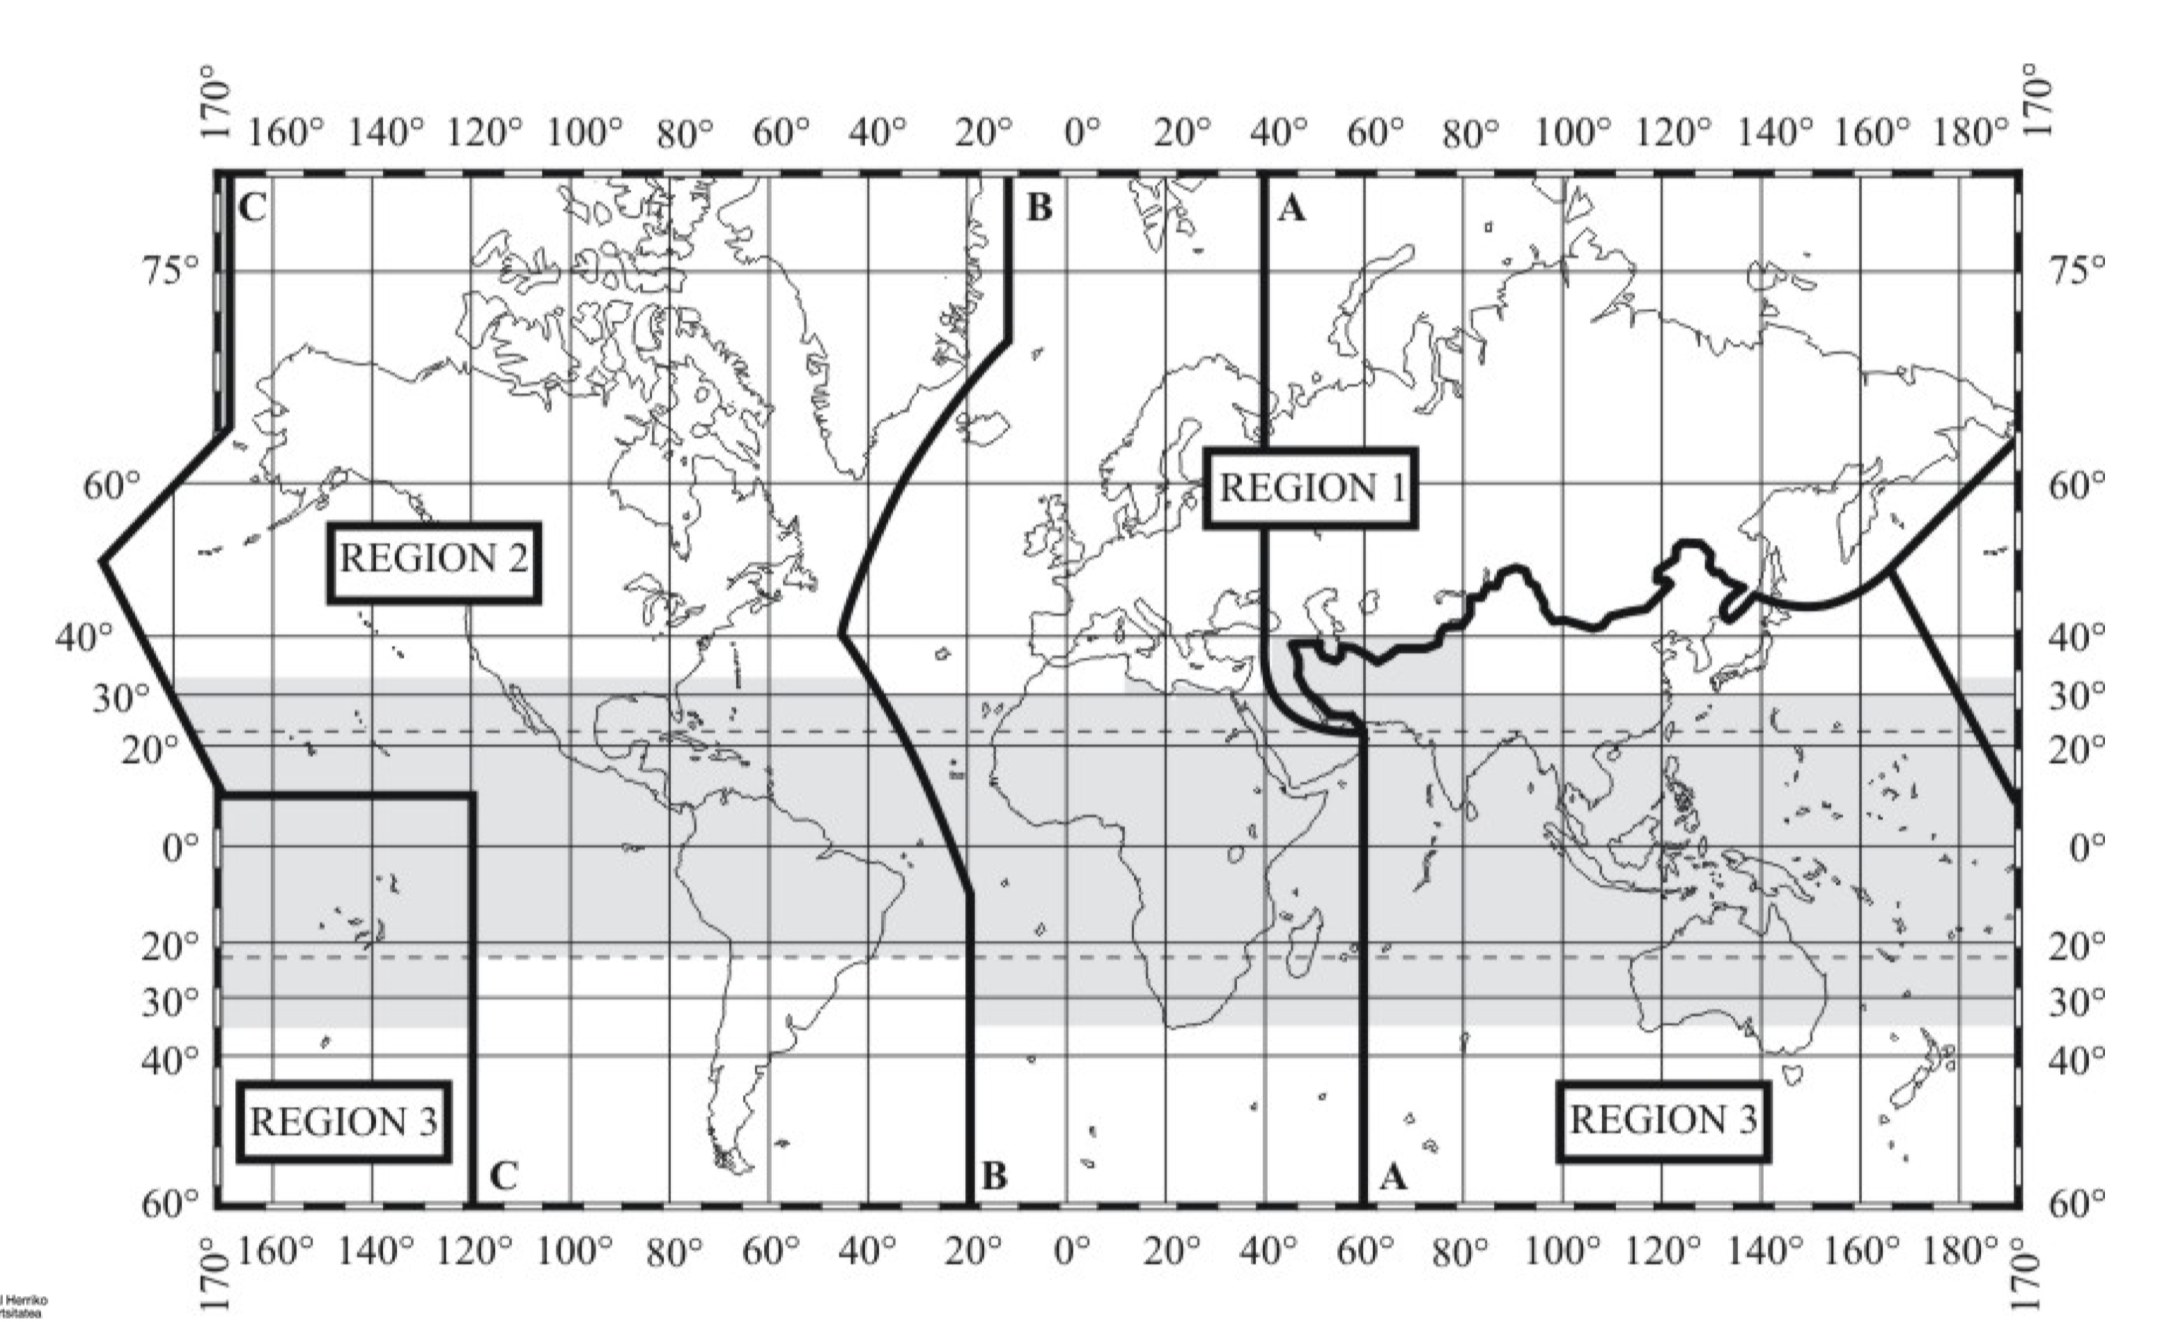
\includegraphics[width=0.5\textwidth]{Regiones}
      \caption{Regiones de frecuencias}
      \label{fig:Regiones de frecuencias}
  \end{figure}

Hay varios \textbf{tipos} de atribuciones de frecuencias:

	\begin{itemize}
		\item \textbf{Exclusiva}: Atribución para un servicio de radio.
		\item \textbf{Compartido}: Atribución para varios servicios de radio.
	\end{itemize}
	
\textbf{Categorías} de servicios:

	\begin{itemize}
		\item \textbf{Primarios}: Prioridad en la elección de las frecuencias, escrito en mayúsculas.
		\item \textbf{Secundario}: No pueden producir interferencias a estaciones primarias. No pueden reclamar protección por interferencia a estaciones de servicios primarios. Pueden reclamar protección contra interferencias de estaciones del mismo servicio u otros servicios secundarios.
	\end{itemize}
	
La \textbf{gestión del espectro} refleja muchas actividades: Planificación del uso del espectro, atribución y asignación de licencias del espectro, interacción con organizadores regionales e internacionales... Históricamente, los reguladores han asignado las frecuencias emitiendo licencias a usuarios específicos para usos específicos $\rightarrow$ Método Administrativo. Hay formas más flexibles de licencia, las bandas se pusieron a disposición de varios usos en vez de sólo para uno y se introdujeron subastas para asignar los espectros a los usuarios.\\

El \textbf{modelo administrativo} es el utilizado por la mayoría de reguladores en el mundo. Los reguladores son las autoridades centrales para la asignación del espectro y decisiones de uso. Las decisiones de asignación son a menudo estáticas en dimensiones temporales y espaciales, es decir, son válidas para períodos de tiempo muy largos y para grandes regiones geográficas por lo que no resulta muy eficiente.\\

El \textbf{modelo de mercado} dice que los recursos del espectro de radiocomunicación debería ser tratado como propiedad privada. La asignación debe de er implementada por las fuerzas de mercado. Los propietarios del espectro deberían ser capaces de comerciar esas partes en mercados secundarios. Los propietarios de espectro podrán utilizar su banda de la manera que quieran a través de cualquier tecnología.\\

La \textbf{teoría del espectro libre} proporciona acceso libre a cualquier espectro para cualquier uso, está necesitada de regulaciones para poner orden.\\

A vistas de \textbf{futuro} se preveé una mayor demanda del espectro disponible, planes centrados en incrementar la compartición del espectro entre servicios, planes centrados en la liberación del espectro no utilizado o no utilizado eficientemente.\\

Las \textbf{licencias} se asignan a estaciones de radio para usuarios específicos con usos específicos y asignadas en subastas. El espectro \textbf{sin licencia} tiene frecuencias para aplicaciones ISM y SDR, limitando la potencia emitida, cualquiera puede transmitir sin una licencia mientras cumpla con las reglas para limitar/evitar interferencias, las principales bandas sin licencias fueron aquellas diseñadas como industriales, científicas y médicas (ISM). En los últimos 15 años ha crecido la demanda en el uso del espectro sin licencia.

\hrulefill

\section{\underline{2. Tecnologías Básicas de Radio}}

\subsection{Bloques de un sistema de radiocomunicación genérico}

\begin{figure}[h]
	\centering
     \begin{tikzpicture}
 	\node at (0,0) [circle,draw] (Antena1) {Antena};
        \node at (3,0) [rectangle,draw] (Medio) {Medio};
        \node at (6,0) [circle, draw] (Antena2) {Antena};
        \node at (0,-2) [rectangle, draw] (Transmisor){Transmisor};
        \node at (3,-2) [rectangle,draw] (Perturbaciones){Perturbaciones};
        \node at (6,-2) [rectangle, draw] (Receptor){Receptor};
        \node at (0,-4) [circle,draw](Fuente)  {Fuente};
        \node at (6,-4) [circle,draw](Display) {InfoDisplay};
        
        
        \draw[->, blue, thick] (Fuente) -- (Transmisor);
        \draw[->, blue, thick] (Transmisor) -- (Antena1);
        \draw[->, red, thick] (Antena1) -- (Medio);
        \draw[->, red, thick] (Medio) -- (Antena2);
        \draw[->, blue, thick] (Receptor) -- (Display);
        \draw[->, blue, thick] (Perturbaciones) -- (Receptor);
        \draw[->, blue, thick] (Perturbaciones) -- (Transmisor);
        \draw[->, blue, thick] (Perturbaciones) -- (Medio);
        \draw[->, blue, thick] (Antena2) -- (Receptor);
        
	\node at (3,-4) [blue] {Señal};
	\node at (3,-4.3) [red]{Radiación};

	\end{tikzpicture}
      \caption{Esquema general}
  \end{figure}

\subsection{Codificación, Entrelazado y Modulación}

\textbf{Codificación}: En cualquier comunicación digital surgen errores cuando algunos de los bits son recibidos con el valor incorrecto. La codificación de canal o FEC (Forward Error Correction) permiten detectar y corregir bits erróneos añadiendo bits redundantes a los bits de datos.

	\begin{equation*}
		\text{Code Rate} = \frac{\text{Bits de datos}}{\text{Bits totales}}
	\end{equation*}

\textbf{Entrelazado}:  Mezclar los bits en el codificador para reordenarlos en el receptor. Si los errores ocurren en ráfagas, los bits erróneos están menos uniformemente distribuidos al entrelazarlos. El inconveniente que tienen es el tiempo de latencia ya que el receptor tiene que esperar a que todos los bits lleguen para decodficarlos.\\

\textbf{Modulación}: Proceso de transferencia de información en banda base a la frecuencia del canal generada por el oscilador. Puede ser modulación en amplitud, fase o frecuencia.\\

\textbf{Filtrado del Canal}: Controlar el solape de los espectros adyacentes y reducir la interferencia entre símbolos (ISI), producida por la limitación del ancho de banda. Esto se consigue haciendo que la función de transferencia del filtro del canal es lo más cercana posible a la respuesta en frecuencia de Nyquist.\\

\textbf{Filtrado de Canal}: Por el teorema de Nyquist se requiere, teóricamente, un mínimo de ancho de banda para detectar $R$ símbolos/s, sin ISI, es R/s Hz. Esto ocurre cuando la función de transferencia del sistema es rectangular y constante entre 0 y $1/2 \cdot T$.

\textbf{TERMINAR}

\subsection{Transmisor}

Toma la señal IF modulada y la lleva al canal de RF y la amplifica para llegar al nivel de potencia requerido para ser transmitida. Normalmente se añade un filtro de canal RF en la etapa final para evitar radiar señales indeseadas. Los amplificadores de potencia son muy sensibles a la potencia reflejada por lo que es necesaria una adaptación de impedancias la antena transmisora. Hay sensores que miden la potencia reflejada y en el caso de la desadaptación de impedancias el transmisor de apaga para evitar daños. También los amplificadores de potencia son responsables de la degradación de la señal transmitida debido a la no linealidad. A la hora de diseñar transmisores hay que jugar con la eficiencia y la degradación de la señal.

\subsection{Antenas}

Son los elementos que adaptan las ondas guiadas, que son transmitidas por cable o guías a las ondas de radio que se propagan por el espacio, añadiendo características direccionales. Son las partes en los sistemas de telecomunicación encargadas de radiar o recibir las ondas electromagnéticas.\\
Normalmente las antenas son clasificadas de acorde a su geometría:

	\begin{itemize}
	\item \textbf{Antenas Lineales o de Cable}: Formadas por una varilla o cables. Los campos radiados se calculan por la corriente que circula por el cable.
	\item \textbf{Anenas de Apertura}: Formadas por una abertura en la cual se produce la radiación. Los campos radiados se calculan por los campos en la abertura. Dependiendo de cómo son generados los campos en la abertura se distinguen 5 antenas: bocinas, reflectoras, lentes, slots y patches.
	\item \textbf{Array de Antenas}: Formadas por un grupo de antenas operando como si fueran una única. Los patrones de radiación dependen principalmente en la disposición del array en lugar del diagrama de radiación de cada antena. Normalmente, las antenas son iguales pero en algunos casos pueden ser diferentes (Yagi o logperiódicas).
	\end{itemize}
	
Para analizar los \textbf{parámetros} que definen las características de una antena hay que tener en cuenta el \textbf{teorema de reciprocidad} que dice que las antenas tienen las mismas características estén transmitiendo o recibiendo.

	\begin{itemize}
		\item \textbf{Impedancia}: La antena será la última parte del sistema de transmisión y el amplificador de transmisión la verá como una carga. La antena es equivalente a una impedancia que disipa potencia generada en el generador. Esa potencia no es disipada sino radiada. Para maximizar la potencia transmitida, la impedancia del a antena y el transmisor de potencia deben estar adaptadas. La impedancia de entrada de la antena ($Z_{in}$, $Z_{a}$ o $Z_{en}$) es definida en los terminales de la antena como el cociente entre voltaje y corriente. En general, consiste en una parte real $R_{in}(f)$ y una parte imaginaria $X_{in}(f)$ $\rightarrow Z_{in}(f) = R_{in}(f) + j \cdot X_{in}(f)$. Si $Z_{in}(f)$ no tiene parte reactiva en alguna frecuencia en concreto ($X_{in} = 0$) se conoce a la antena como antena resonante para esa frecuencia.
		
			\begin{equation*}
			\eta_{l} = \frac{P_{r}}{P_{in}} = \frac{R_{r}}{R_{r} + R_{\omega}}
			\end{equation*}
			
			\begin{center}
\begin{circuitikz}[scale=.5, transform shape, european]

	\draw (0,0) 
		to[R  = $R_{\Omega}$] (2,0)
		to[R  = $jX_{in}$] (4,0)
		-- (5,0)
		to[R  = $R_{r}$] (5,-2)
		-- (0,-2);
		
	\draw[-latex] (-.2,-2) -- (-.2,0) node[left] {$V_{in}$};
	\draw[-latex] (0, -.5) -- (1,-.5) node[below] {$I_{in}$};	
\end{circuitikz}
\end{center}
	
		\begin{equation*}
			P_{in} = |I_{in}|^{2} (R_{r} + R_{\Omega}) \hspace{20pt} P_{r} = |I_{in}|^{2} R_{r}
		\end{equation*}

		El circuito equivalente para TX y RX de la antena es
		
		\begin{center}
			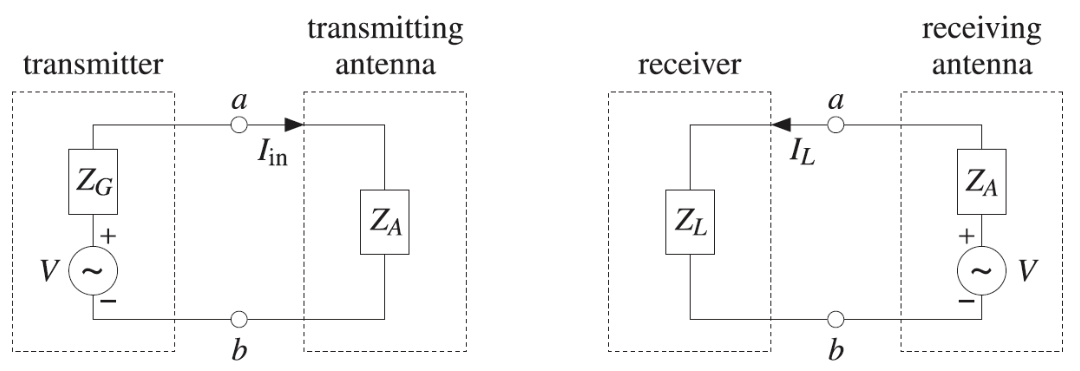
\includegraphics[width = .35\textwidth]{TXRX}
		\end{center}
		
		En RX, $V$ es la tensión en circuito abierto de la antena receptora. $V$ es la tensión en circuito abierto de la antena receptora, depende del campo $E$ o densidad de potencia en la localización de la antena y características de ésa. SI $Z_{A} \neq Z_{L}$ las pérdidas por desadaptación reducen la potencia en $Z_{L}$.
		
		\item \textbf{Impedancia}: Indica si un dispositivo puede ser utilizado como antena o no. La impedancia se puede calcular mediante el coeficiente de reflexión:
			\begin{equation*}
				\rho = \frac{Z_{in} - Z_{o}}{Z_{in} + Z_{o}}
			\end{equation*}
			
		Los analizadores de espectros dan el valor de $Z_{in}$ directamente. Otras medidas relacionadas con $Z_{in}$ y $\rho$ son las \textbf{pérdidas de retorno}:
			\begin{equation*}
				-20 \cdot \log |\rho|
			\end{equation*}
			
		\textbf{COE} (Coeficiente de Onda Estacionaria):
		
			\begin{equation*}
				\text{COE} = \frac{1 + |\rho|}{1 - |\rho|}
			\end{equation*}
		\textbf{Pérdidas por desadaptación}:
		
			\begin{equation*}
				10 \log (1 - |\rho|^{2})
			\end{equation*}
			
		En transmisión, una desadaptación entre el transmisor y la antena puede causar grandes daños en el equipamiento debido a la potencia reflejada.
		
		\item \textbf{Far field radiation region}:A una distancia suficientemente grande de la antena la energía se radia de forma esférica y los frentes de onda pueden ser considerados planos, los campos $\vec{E}$ y $\vec{H}$ son mutuamente \textbf{perpendiculares}, perpendiculares a la dirección de propagación $\wedge{r}$ y sus módulos están en fase y relacionados con la impedancia intrínseca del medio:

	\begin{equation*}
		\frac{|\vec{E}|}{|\vec{H}|} = \eta
	\end{equation*}
	
La distancia a la cual los campos radiados son considerados como ondas planas y los parámetros de radiación son constantes dependen de la antena y frecuencia. Esta región del espacio se llama far field radiation region. Un valor aproximado para la mínima distancia que asegura la condición far field es:

	\begin{equation*}
		r > \frac{2 D^{2}}{\lambda} \text{D: Largest dimension of the antenna}
	\end{equation*}

	\textbf{Densidad de Flujo por Unidad de Área}: O Densidad de potencia obtenida del campo eléctrico y magnético como (rms):
	
		\begin{IEEEeqnarray*}{rCl}
			\vec{W} (\theta, \phi) = \vec{S} (\theta, \phi) & = &  Re \left( \vec{E} x \vec{H} \right) W/m^{2} \\
							   \vec{S} (\theta, \phi) & = & \frac{1}{\eta} \left[ \left| \vec{E}_{\theta} (\theta, \phi) \right|^{2} + \left| \vec{E}_{\phi} (\theta, \phi) \right|^{2} \right]	 \hat{r}
		\end{IEEEeqnarray*}

		Este vector es el valor RMS del vector Poynting. La potencia radiada puede ser calculada como la integral del flujo de potencia a través de una superficie que engloba a la antena:
		
		\begin{equation*}
			P_{r} = \iint_{S} \vec{S} (\theta, \phi) \cdot \partial \vec{s} = \int_{0}^{2\pi} \int_{\theta = 0}^{\phi = \pi} \vec{S} (\theta, \phi) \hat{r} \cdot sin^{2} \cdot  \theta \partial \theta \cdot \partial \phi
		\end{equation*}
	
		\item \textbf{Patrón de Radiación o Patrón de Antena}: Gráfico tridimensional de una de las siguientes magnitudes.

			\begin{IEEEeqnarray*}{rCl}
				\text{Intensidad de Campo Eléctrico Normalizada}&:& 20 \cdot \frac{\left| \vec{E} (\theta, \varphi) \right|}{|\vec{E}_{\text{max}} |} \\
				\text{Densidad de Potencia Radiada Normalizada}&:& 10 \cdot \log \frac{S_{rad} (\theta, \varphi)}{S_{rad_{max}}}
			\end{IEEEeqnarray*}

		Debido a las propiedades de las ondas planas ambos diagramas son iguales y el campo magnético puede ser usado con el mismo resultado. El patrón de radiación es un gráfico que ayuda a visualizar dónde transmite/recibe potencia la antena.

	\end{itemize}

\hrulefill

	
	
	
%\vfill




%\end{multicols}

\end{document}